\providecommand{\mainpath}{..} % Command to retrieve the path of the main file. It must be defined before documentclass.

\documentclass[\mainpath/main]{subfiles}
\begin{document}

\chapter{Architectural Design}
\label{architectural_design}

% Command to be executed after the starting of every chapter
\setmyfancystyle
% ----------------

In this chapter the complete architecture of myTaxiService is shown with various levels of description. In the \autoref{ArchitecturalDesign:high_level} there is a global view and the interactions between all the components are described.\\ 
The data tier is illustrated in \autoref{ArchitecturalDesign:component} with all related policies and entities. Then the other tiers are characterized using different diagrams.\\
In the \autoref{ArchitecturalDesign:deploy} the deployment of each components is illustrated (for instance the data component is sit in a different place with respect to the other component? It is replaced twice or more? And similar question will have an answer).\\
In \autoref{ArchitecturalDesign:runtime} the view level is defined. The interactions between all kinds of user and the system are described using UX diagrams and sequence diagrams that display the order in which each screen is visualized. Besides, the mockups of these screens are shown in %\autoref{UI}.
\\
A standalone paragraph, the \autoref{ArchitecturalDesign:comp_interfaces}, is dedicated to list all interfaces, both internal (between two components) and external.\\
Finally, in the \autoref{ArchitecturalDesign:design_patterns} the design patterns used to develop myTaxiService are described first in general case. After that, all the changes needed to adapt this design patterns to our system are characterized.


\section{Distinctions between various kind of Users and Clients}
\label{ArchitecturalDesign:preamble}
The "visible architecture" of myTaxiService is very varied. The term visible is referred to various user interfaces, so what the users can see when they are using the system.\\
On the other hand, we have said that myTaxiService is varied because it has two principal version (MA and WS) and for both of them there are a few levels of specialization, according to the kind of the user. All of them are explained in this paragraph.\\
\\
The WS version is shown into a browser, so there is no client application that can be used. Hence, all the pages are loaded into the server and then they are sent to the client browser.\\
Instead, the MA is a client application and it has different ways to communicate with the server. All the aspects concerning these differences are explained better during the descriptions of the architecture's components that handle the clients.\\
\\
%Fare un riferimento al capitolo che mette in relazione RASD e DD per far capire il tipo di attore?
The cab company is the special user who administrates the service. Obviously, it has a command center at its headquarters where it can control both the system and the service situation. Hence its special functions are not implemented neither in the MA nor in the WS, but they can directly access the server using private keys and reserved terminals.\\
A customers can use both the MA and the WS to enjoy his functionalities. No particular cases or restriction are reserved to them.\\
When a driver logs into the service, we suppose that it is working, so his special functionalities are developed and implemented only for the MA. In fact no driver carries a computer with an internet connection on his taxi and uses it. On the other hand, since the driver is also an user, it can use the WS, but here he has only the user functionalities due to the reason shown above.\\



\section{High level components and their interaction}
\label{ArchitecturalDesign:high_level}

The main structure of myTaxiService can be described as a Service-Oriented architecture (see \autoref{ArchitecturalDesign:design_patterns} to have a detailed description of this design pattern). In addition to this idea the Model-View-Control paradigm is applied in order to develop a good-programmed, reusable and easy-maintainable system.
\begin{figure}[h]
	\label{ArchitecturalDesign:figure1}
	\centering
	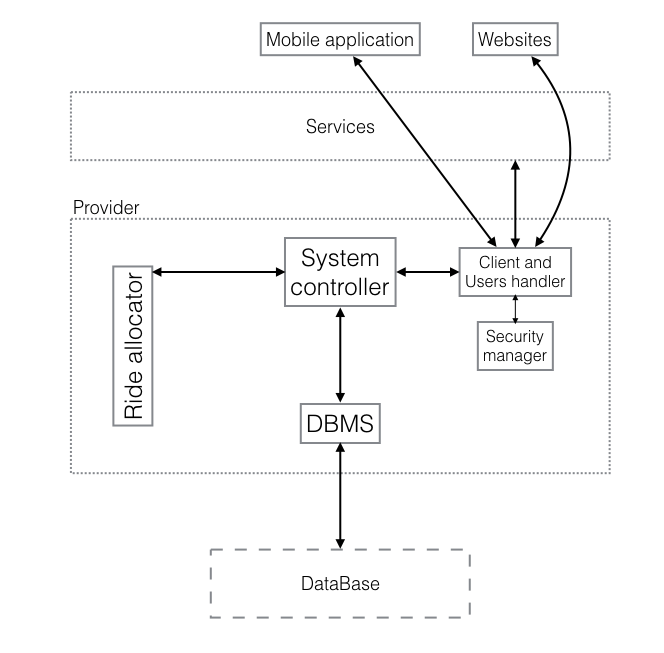
\includegraphics[width=10cm] {main_architecture}
	\caption{High level architecture}
\end{figure}

In the \ref{ArchitecturalDesign:figure1} is shown the architecture. At the bottom of the figure there is the \nameref{ArchitecturalDesign:datatier} which contains only the database (a component that stores all data about the customers, the rides and the system).\\
\\
The central part of the picture contains the provider, the big component that gives the service. At this level of description we can look in the provider. This component is splitted into five parts. The DataBase Managment System (DMBS) manages all communications with the \nameref{ArchitecturalDesign:datatier}. The Ride Allocator has only one role, to assign and to handle the ride, both future and zerotime. The system controller is the \textquotedblleft heart\textquotedblright of the provider: it involves the ride allocator when is needed, it gives all the services of the system, it provides the DBMS with the data to be stored (or asks him some data to be found) and, communicate with the Client and Users Handler. The Client and User Handler, as its name said, handles the communications with the clients and administrates the Uses, so which services can be shown and selected by them.\\
\\
The third tier is a presentation level. In the Service-Oriented pattern this level represents the presentation of available services. Here, the clients can see the services and select the desired one.\\
Finally, at the top of the image, there is a representation of the two kind of clients, the Ws and the MA.\\
\\
All the tiers are also distinguished into the three parts of MVC-paradigm. The \nameref{ArchitecturalDesign:datatier} is the model\footnote{see the Alloy section or the UML class diagram into the RASD to see it. However, in section \ref{ArchitecturalDesign:datatier} it is studied again.}. The provider is also the controller: even if the controller can be see as the component that manages the interaction between the view and the model, in this application we consider other \textquotedblleft handler\textquotedblright as part of controller because they encapsulate rules and action codes. The view is the union between the presentation tier (here the services are only shown to client, the \textquotedblleft decisions\textquotedblright are taken by the provider) and the clients.\\
\\
Up to now, we have introduced all the main components or tier of our system, without focus on the communications between them, so we'll dedicate a little part of this paragraph on this argument.\\
All the communications between the model and the provider are managed by the DBMS that has store policies and finds the required data. The system controller is the central node in communication because it is the only way to all other component of the provider.
The Client and User Handler is the link between the provider and the clients. It checks the type of the current user and, as consequence, the available services that he can uses. When a user asks a service, he binds the request asking for the related function it the System Controller. Finally, it checks the type of client, because they have two ways of communication. When a user is connected with the WS, the Client and User Handler load the pages into itself and then, using the HTTPS protocol sent them to the client. Besides, the communications with the MA is implemented using sockets. The implementation of these ways of communication with the clients is realized by a common interface (see the section \ref{ArchitecturalDesign:comp_interfaces} for further information).

\section{Component view}
\label{ArchitecturalDesign:component}


\subsection{Data Tier}
\label{ArchitecturalDesign:datatier}


TESTO NON UFFICIALE\\
qui si descrivono nel dettaglio tutti i vari componenti, specialmente il data tier e il server tier. 

\section{Deployment view}
\label{ArchitecturalDesign:deploy}

$TESTO NON UFFICIALE\\
Distribuzione dei vari component\\
Ci sono più macchine per il server? Ci sono altri componenti come firewall? ecc$

\section{Runtime view}
\label{ArchitecturalDesign:runtime}

TESTO NON UFFICIALE\\
qui si pone particolare attenzione alle screen e quindi al client tier.\\
Tutti i sequence diagram e gli UX saranno messi qui\\

\section{Component Interfaces}
\label{ArchitecturalDesign:comp_interfaces}

TESTO NON UFFICIALE\\
descrizione di tutte le interfacce tra i vari component e verso l'esterno.\\
Forse si metteranno anche i principali metodi?\\


\section{Selected architectural styles and patterns}
\label{ArchitecturalDesign:design_patterns}


EVENTBASED per ora\\


%End of chapter
\end{document}